\documentclass[11pt,table]{book}
\usepackage{lipsum}
\usepackage[ISBN=978-80-86619-23-1]{ean13isbn}


\usepackage[utf8]{inputenc}
\usepackage{graphicx}
\usepackage{listings}
\usepackage{lmodern}
\usepackage[T1]{fontenc}
\usepackage{libertine}
\usepackage{tikz}
\usetikzlibrary{fit,arrows,shapes,backgrounds}
\usepackage{emselip}
\widowpenalty10000
\clubpenalty10000
\brokenpenalty=10000

\usepackage{comment}
\usepackage{float}
\usepackage{microtype}

\usepackage{etoolbox}

% definit un booleen pour inclure ou non les corrections
% par defaut a true
\newtoggle{includematlabcorrection}
\toggletrue{includematlabcorrection}
\newtoggle{includepythoncorrection}
\toggletrue{includepythoncorrection}
\newtoggle{matlabbook}
\toggletrue{matlabbook}
\newtoggle{pythonbook}
\toggletrue{pythonbook}


\newcommand{\inputmatlabcorrection}[1]{\iftoggle{includematlabcorrection}{\input{#1}}{}
}
\newcommand{\inputpythoncorrection}[1]{\iftoggle{includepythoncorrection}{\input{#1}}{}
}
\newcommand{\ifmatlab}[1]{\iftoggle{matlabbook}{#1}{}
}
\newcommand{\ifpython}[1]{\iftoggle{pythonbook}{#1}{}
}

\newcommand{\matlabregistered}{MATLAB\textsuperscript{\textregistered}}
\usepackage{xcolor}

\definecolor{dkgreen}{rgb}{0,0.6,0}
\definecolor{gray}{rgb}{0.5,0.5,0.5}
\definecolor{mauve}{rgb}{0.58,0,0.82}
% colors
\definecolor{darkblue}{rgb}{0,0.1,0.5}
\definecolor{blueemse}{RGB}{0 63 135} % bleu pantone 294 CV / EMSE
\definecolor{ocre}{RGB}{243,102,25} % Define the orange color used for highlighting 
\definecolor{matlabblue}{RGB}{34 85 139} % bleu fenetre matlab

%*******************************************************************************
% couleurs automne
\definecolor{automne_primaire0}{RGB}{ 95, 57, 65}
\definecolor{automne_primaire1}{RGB}{208,193,196}
\definecolor{automne_primaire2}{RGB}{152,112,121}
\definecolor{automne_primaire3}{RGB}{86, 21, 35}
\definecolor{automne_primaire4}{RGB}{64,  0, 14}

\definecolor{automne_complement0}{RGB}{ 66, 89, 54}
\definecolor{automne_complement1}{RGB}{187,196,182}
\definecolor{automne_complement2}{RGB}{119,143,106}
\definecolor{automne_complement3}{RGB}{ 41, 81, 19}
\definecolor{automne_complement4}{RGB}{ 21, 60,  0}

%%% couleurs a utiliser
% code informatique
\colorlet{c_code_numberstyle}{gray} % numerotation de lignes
\colorlet{c_code_keyword}{blueemse} % keyword
\colorlet{c_code_rule}{automne_primaire4} % lignes
\colorlet{c_code_comment}{red} % commentaires
\colorlet{c_code_string}{automne_primaire0} % chaines de caracteres
\colorlet{c_code_colback}{automne_primaire1!10} % fond des fenetres
\colorlet{c_code_colframe}{automne_primaire3} % bordure des fenetres
\colorlet{c_code_icon_fill}{automne_primaire1} % icone: fond
\colorlet{c_code_title}{automne_primaire3} % titre (non utilise)

% fenetres de questions
\colorlet{c_qbox_colback}{automne_primaire1} % fond des fenetres
\colorlet{c_qbox_colframe}{automne_primaire4} % bordure des fenetres
\colorlet{c_qbox_icon_colback}{automne_primaire1!10} % icone: fond
\colorlet{c_qbox_icon_colframe}{automne_primaire3} % icone: bordure

% document
\colorlet{c_title}{automne_complement4}
\colorlet{c_rule}{automne_complement4}
\colorlet{c_page}{automne_complement4}
\colorlet{c_section}{automne_complement4}
\colorlet{c_section_colframe}{automne_complement4} % bordure des fenetres
\colorlet{c_section_colback}{automne_complement1}  % fond des fenetres

% %***************************************************************************
% % % couleur vert orange flashy
% \definecolor{flashy_primaire0}{RGB}{127,234,110 }
% \definecolor{flashy_primaire1}{RGB}{232,255,229}
% \definecolor{flashy_primaire2}{RGB}{172,248,160}
% \definecolor{flashy_primaire3}{RGB}{ 92,207, 74}
% \definecolor{flashy_primaire4}{RGB}{ 58,136, 46}
% 
% \definecolor{flashy_complement0}{RGB}{160, 61, 68}
% \definecolor{flashy_complement1}{RGB}{252,140,148}
% \definecolor{flashy_complement2}{RGB}{228,111,120}
% \definecolor{flashy_complement3}{RGB}{103, 28, 33}
% \definecolor{flashy_complement4}{RGB}{ 43,  7, 10}
% %%% couleurs a utiliser
% % code informatique
% \colorlet{c_code_numberstyle}{gray}
% \colorlet{c_code_keyword}{blueemse}
% \colorlet{c_code_rule}{flashy_primaire4}
% \colorlet{c_code_comment}{red}
% \colorlet{c_code_string}{flashy_primaire0}
% \colorlet{c_code_colback}{flashy_primaire1!10} % fond des fenetres
% \colorlet{c_code_colframe}{flashy_primaire3} % bordure des fenetres
% \colorlet{c_code_icon_fill}{flashy_primaire1}
% \colorlet{c_code_title}{flashy_primaire3}
% 
% % fenetres de questions
% \colorlet{c_qbox_colback}{orange!10} % fond des fenetres
% \colorlet{c_qbox_colframe}{flashy_primaire3} % bordure des fenetres
% \colorlet{c_qbox_icon_colback}{orange!20}
% \colorlet{c_qbox_icon_colframe}{flashy_primaire3}
% 
% % document
% \colorlet{c_title}{flashy_complement3}
% \colorlet{c_rule}{flashy_complement3}
% \colorlet{c_page}{flashy_complement4}
% \colorlet{c_section}{flashy_complement4}
% \colorlet{c_section_colframe}{flashy_complement4} % bordure des fenetres
% \colorlet{c_section_colback}{flashy_complement2}  % fond des fenetres


\usepackage{pdfpages}

\usepackage[%           % Fine in most cases
            pdfpagelabels,hypertexnames=true,
            plainpages=false,
            naturalnames=false,
            pdftitle={Image Processing Tutorials},
				backref=page,
				linktoc=all,
				hidelinks
  			]{hyperref}

\hypersetup{colorlinks,
            linkcolor=c_section,
            anchorcolor=c_section,
            citecolor=c_section}

    
\usepackage{import}
%\subimport{./}{couleurs.tex}
\usepackage{tikz}
\usetikzlibrary{arrows,calc,shapes.geometric,plotmarks}
\usepackage{listings}
\usepackage{tcolorbox}
\tcbuselibrary{listings,skins,breakable}


\usepackage{accsupp}
\newcommand{\noncopynumber}[1]{%
    \BeginAccSupp{method=escape,ActualText={}}%
    #1%
    \EndAccSupp{}%
}


\lstdefinestyle{MatlabStyle} { %
  language=Matlab,                % the language of the code
%  float,
%  floatplacement=htbp,
  basicstyle=\footnotesize,           % the size of the fonts that are used for the code
  numbers=left,                   % where to put the line-numbers
  numberstyle=\tiny\color{c_code_numberstyle}\noncopynumber,  % the style that is used for the line-numbers
  stepnumber=2,                   % the step between two line-numbers. If it's 1, each line 
                                  % will be numbered
  numbersep=5pt,                  % how far the line-numbers are from the code
  %backgroundcolor=\color{white},      % choose the background color. You must add \usepackage{color}
  showspaces=false,               % show spaces adding particular underscores
  showstringspaces=false,         % underline spaces within strings
  showtabs=false,                 % show tabs within strings adding particular underscores
  %frame=single,                   % adds a frame around the code
  %rulecolor=\color{blueemse},        % if not set, the frame-color may be changed on line-breaks within not-black text (e.g. commens (green here))
  tabsize=2,                      % sets default tabsize to 2 spaces
  captionpos=b,                   % sets the caption-position to bottom
  breaklines=true,                % sets automatic line breaking
  breakatwhitespace=false,        % sets if automatic breaks should only happen at whitespace
  title=\lstname,         % show the filename of files included with \lstinputlisting;
                                  % also try caption instead of title
  keywordstyle=\color{c_code_keyword},          % keyword style
  commentstyle=\color{c_code_comment},       % comment style
  stringstyle=\color{c_code_string},         % string literal style
  escapeinside={\%*}{*)},            % if you want to add a comment within your code
  morekeywords={*,...},               % if you want to add more keywords to the set
 % literate=*{-}{-}1  
  columns=flexible
}

\lstdefinestyle{PythonStyle}{ %
  language=Python,                % the language of the code
  basicstyle=\footnotesize,       % the size of the fonts that are used for the code
  numbers=left,                   % where to put the line-numbers
%  float,
%  floatplacement=htbp,
  numberstyle=\tiny\color{c_code_numberstyle},  % the style that is used for the line-numbers
  stepnumber=2,                   % the step between two line-numbers. If it's 1, each line 
                                  % will be numbered
  numbersep=5pt,                  % how far the line-numbers are from the code
  %backgroundcolor=\color{white},  % choose the background color. You must add \usepackage{color}
  showspaces=false,               % show spaces adding particular underscores
  showstringspaces=false,         % underline spaces within strings
  showtabs=false,                 % show tabs within strings adding particular underscores
  %frame=single,                   % adds a frame around the code
  rulecolor=\color{c_code_rule},        % if not set, the frame-color may be changed on line-breaks within not-black text (e.g. commens (green here)) 
  tabsize=2,                      % sets default tabsize to 2 spaces
  captionpos=b,                   % sets the caption-position to bottom
  breaklines=true,                % sets automatic line breaking
  breakatwhitespace=false,        % sets if automatic breaks should only happen at whitespace
  title=\lstname,                   % show the filename of files included with \lstinputlisting;
                                  % also try caption instead of title
  keywordstyle=\color{c_code_keyword},          % keyword style
  commentstyle=\color{c_code_comment},       % comment style
  stringstyle=\color{c_code_string},         % string literal style
 % index=[1][meshgrid],
  escapeinside={\%*}{*)},            % if you want to add a comment within your code
  morekeywords={*,...},               % if you want to add more keywords to the set
  tabsize=3,
  literate=*{-}{-}1
}
% \lstnewenvironment{matlab}
%   {\lstset{language=Matlab,style=MatlabStyle}}
%   {}

\newenvironment{matlab}{%
  \tcblisting{listing only,colback=c_code_colback,colframe=c_code_colframe, enlarge top by=5.5mm,enhanced,breakable,boxrule=1pt,%
     overlay={\node[anchor=west,xshift=10pt,draw=c_code_colframe, line width=2pt, rectangle, rounded corners=2pt,fill=c_code_icon_fill,inner sep=2pt,outer sep=0pt, minimum size=20pt] at (frame.north west) {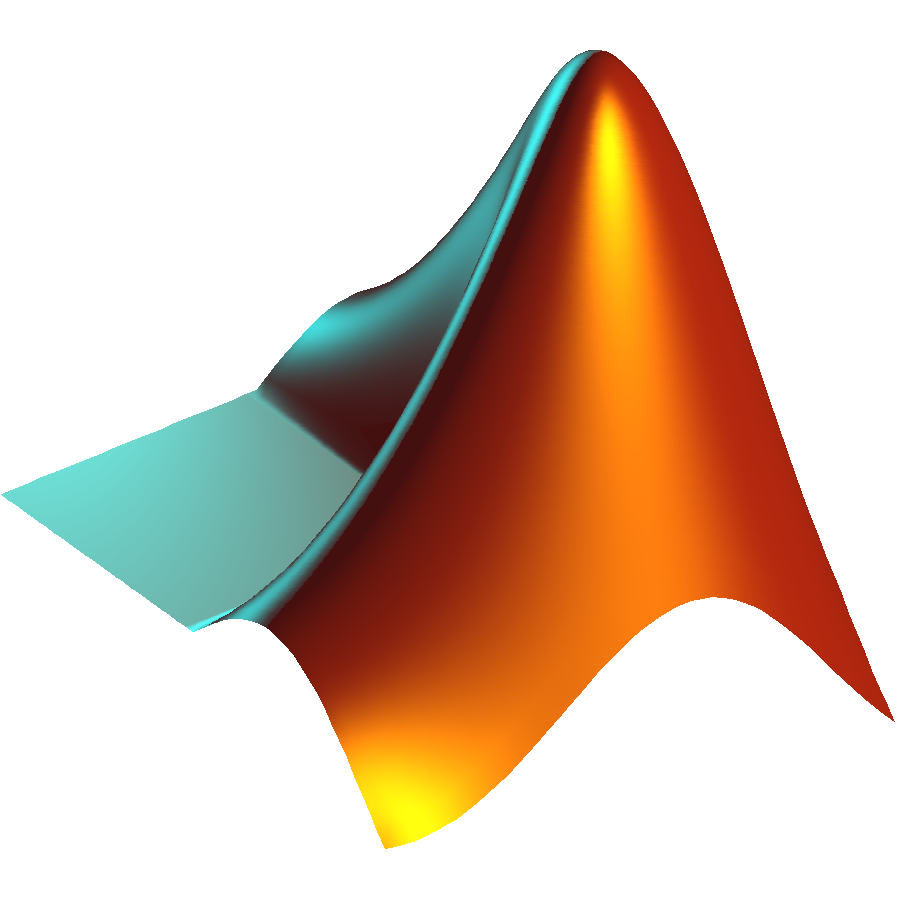
\includegraphics[width=16pt]{matlab-logo.png}};},%
     listing options={basicstyle=\footnotesize\ttfamily,breaklines=true,%
                      postbreak={\mbox{$\hookrightarrow\space$}},%
                      language=Matlab,style=MatlabStyle},%
  }%
 }%
 {\endtcblisting}

\newenvironment{python}{%
  \tcblisting{listing only,colback=c_code_colback,colframe=c_code_colframe, enlarge top by=5.5mm,enhanced,boxrule=1pt,%
     overlay={\node[anchor=west,xshift=10pt,draw=c_code_colframe, line width=2pt, rectangle, rounded corners=2pt,fill=c_code_icon_fill,inner sep=2pt,outer sep=0pt, minimum size=20pt] at (frame.north west) {
\includegraphics[width=16pt]{python-logo.pdf}};},%
     listing options={basicstyle=\footnotesize\ttfamily,breaklines=true,%
                      postbreak={\mbox{$\hookrightarrow\space$}},language=Python,style=PythonStyle},%
  }%
 }%
 {\endtcblisting}
\newenvironment{sh}{%
  \tcblisting{listing only,colback=c_code_colback,colframe=c_code_colframe, enlarge top by=5.5mm,enhanced,boxrule=1pt,%
     overlay={\node[anchor=west,xshift=10pt,draw=c_code_colframe, line width=2pt, rectangle, rounded corners=2pt,fill=c_code_icon_fill,inner sep=2pt,outer sep=0pt, minimum size=20pt] at (frame.north west) {
\includegraphics[width=16pt]{sh-logo.pdf}};},%
     listing options={basicstyle=\footnotesize\ttfamily,breaklines=true,%
                      postbreak={\mbox{$\hookrightarrow\space$}},language=sh,style=PythonStyle},%
  }%
 }%
 {\endtcblisting}


\newcommand{\triangcirc}{\tikz{
\node[circle,white,draw,inner sep=3pt] (c) {};
\node[isosceles triangle,
      white,
      fill,
      rotate=-90,
      anchor=apex,
      isosceles triangle apex angle=60,
      inner sep=1.5pt] (t) at ([yshift=0.5pt]c.south) {};}}
% 
% \makeatletter
% \renewcommand*\thelstnumber{\makebox[3em][r]{\ifnum\value{lstnumber}<10 0\fi\the\value{lstnumber}}}
% \def\three@digits#1{\ifnum#1<10 00\else\ifnum#1<100 0\fi\fi\number#1}
% \makeatother

\newenvironment{mwindow}{%
  \tcblisting{   
  enhanced,
  arc = 0pt,
  outer arc = 2pt,
  colback = white,
  colframe = matlabblue,
   listing only,
  fonttitle = \bfseries,
  listing options = {%
    language = matlab,
    style=MatlabStyle
  },
  overlay = {%
    \fill[gray!30] 
      (interior.north west)
      rectangle 
      ([xshift = 1em]interior.south west);
  },%
%   /utils/exec = {%
%     \def\thelstnumber{%
%       \texttt{\csname three@digits\endcsname{\the\value{lstnumber}}}}},
  title = {\ttfamily Command window\hfill\triangcirc}
  }%
 }%
 {\endtcblisting}

 
  % langage par défaut
\lstset{language=Matlab, style=MatlabStyle}

\def\minline{\lstinline[language=Matlab,breaklines=true]}
\def\pinline{\lstinline[language=Python,breaklines=true]}

%----------------------------------------------------------------------------------------
%	REMARK ENVIRONMENT
%----------------------------------------------------------------------------------------

% Remark with \matlabregistered{} logo
\newenvironment{mremark}{\par\vskip10pt\small % Vertical white space above the remark and smaller font size
\noindent\ignorespaces\begin{minipage}{20pt} 
   \begin{tikzpicture}[overlay]
   \node[anchor=east,draw=c_code_colframe, line width=1pt, rectangle, rounded corners=2pt,fill=c_code_icon_fill,inner sep=2pt,outer sep=0pt, minimum size=20pt] at (-10pt,0pt){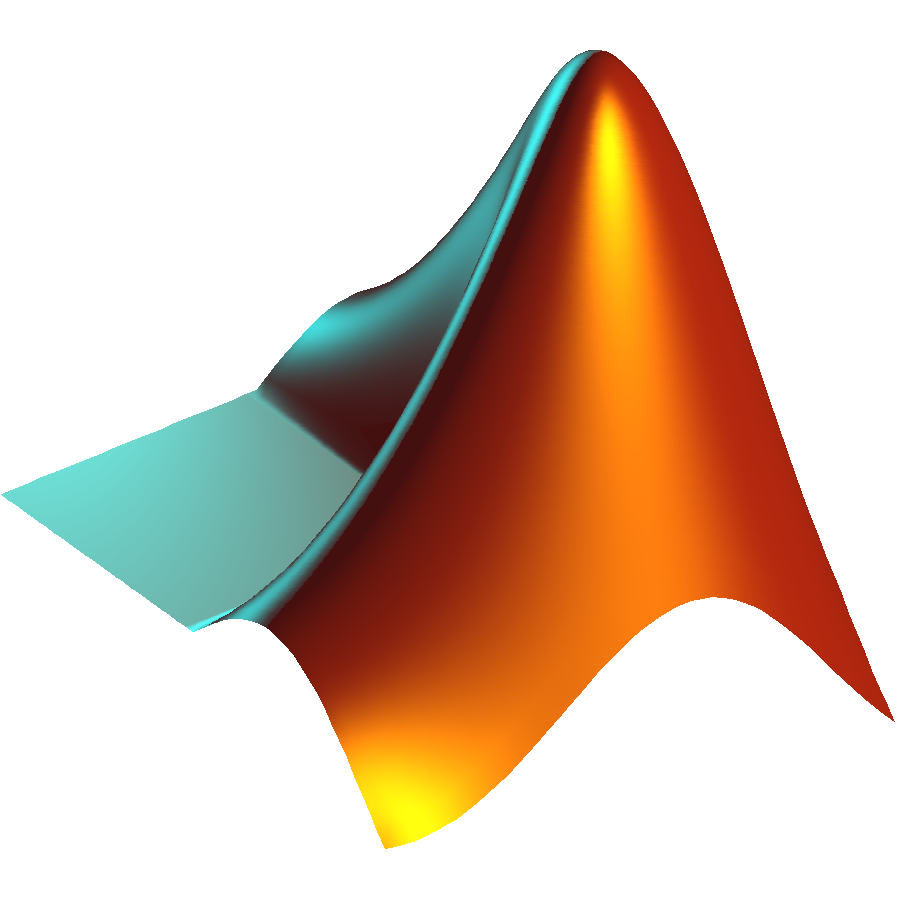
\includegraphics[width=16pt]{matlab-logo.png}};
   \end{tikzpicture}%
  \end{minipage}%
	\begin{minipage}{.8\textwidth}\flushleft
  }
{
\end{minipage}\par\noindent%
\ignorespacesafterend
\vskip12pt} % Tighter line spacing and white space after remark

% Remark with python logo
\newenvironment{premark}{\par\vskip10pt\small % Vertical white space above the remark and smaller font size
\noindent\ignorespaces\begin{minipage}{20pt}   
   \begin{tikzpicture}[overlay]
   \node[anchor=east,draw=c_code_colframe, line width=1pt, rectangle, rounded corners=2pt,fill=c_code_icon_fill,inner sep=2pt,outer sep=0pt, minimum size=20pt] at (-10pt,0pt){
\includegraphics[width=16pt]{python-logo.pdf}};
   \end{tikzpicture}%
  \end{minipage}%
	\begin{minipage}{.8\textwidth}\flushleft
  }
{
\end{minipage}\par\noindent%
\ignorespacesafterend
\vskip12pt} % Tighter line spacing and white space after remark


\newtcolorbox{qbox}[1][]{
	enhanced jigsaw,
  %width=0.5\textwidth,  %% change
  colback=c_qbox_colback,
  colframe=c_qbox_colframe,
  title={
\includegraphics[width=10pt]{interrogation.pdf}},
  boxrule=2pt,
  breakable,
  %left=10pt,right=10pt,top=20pt,bottom=20pt,
  attach boxed title to top left= {xshift=10pt,yshift*=-\tcboxedtitleheight/2},
  boxed title style={boxrule=0pt,size=small,colback=c_qbox_icon_colback,colframe=c_qbox_icon_colframe},
  before=\par\vspace{3mm},
  #1
}

\newtcolorbox{mhelp}[1][]{
	enhanced jigsaw,
  %width=0.5\textwidth,  %% change
  colback=c_code_colback,
  colframe=c_code_colframe,
  coltitle=c_code_title,
  title={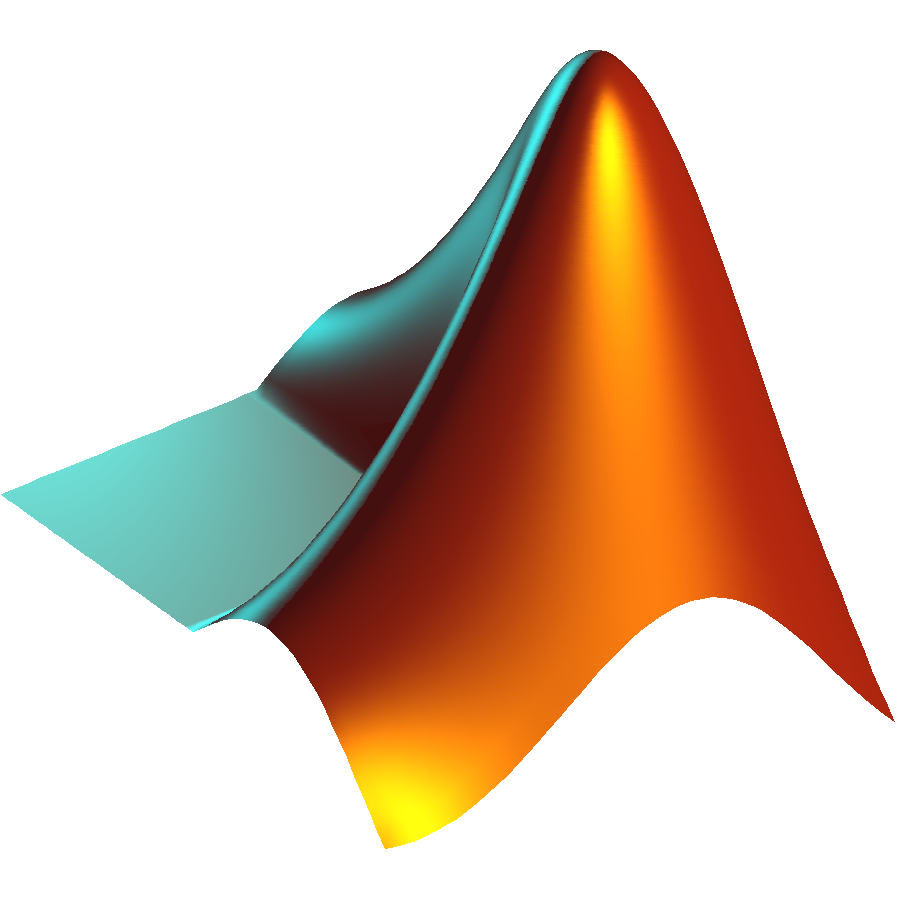
\includegraphics[width=16pt]{matlab-logo.png} Informations},
  boxrule=1pt,
  breakable,
  attach boxed title to top left= {xshift=10pt,yshift*=-\tcboxedtitleheight/2},
  boxed title style={size=small,colback=c_code_colback,colframe=c_code_colframe},
  #1
}


\newtcolorbox{phelp}[1][]{
	enhanced jigsaw,
  %width=0.5\textwidth,  %% change
  colback=c_code_colback,
  colframe=c_code_colframe,
  coltitle=c_code_title,
  title={
\includegraphics[width=16pt]{python-logo.pdf} Informations},
  boxrule=1pt,
  breakable,
  %left=10pt,right=10pt,top=20pt,bottom=20pt,
  attach boxed title to top left= {xshift=10pt,yshift*=-\tcboxedtitleheight/2},
  boxed title style={size=small,colback=c_code_colback,colframe=c_code_colframe},
  #1
}

\usepackage{subfig}

%\usepackage{subcaption}
%\usepackage[table]{xcolor}

% display frame
%\usepackage{showframe}

% maths
\usepackage{amsmath}
\usepackage{amssymb}
\usepackage[cm]{fullpage}
\usepackage[boxed]{algorithm2e}
%\pdfsuppresswarningpagegroup=1

\usepackage{tikz}
\usetikzlibrary{shapes,backgrounds,shapes.misc}
% packages de mise en page
\usepackage[newparttoc]{titlesec} % Allows customization of titles
\usepackage{etoolbox}

%%%%%%%%%%%%%%
% cette partie est due à un bug de texlive
\makeatletter
\patchcmd{\ttlh@hang}{\parindent\z@}{\parindent\z@\leavevmode}{}{}
\patchcmd{\ttlh@hang}{\noindent}{}{}{}
\makeatother

%------------------------------------------------------------------------------
%	MAIN TABLE OF CONTENTS
%------------------------------------------------------------------------------

\usepackage{titletoc} % Required for manipulating the table of contents

\contentsmargin{0cm} % Removes the default margin
% 
% \titleformat{\part}[display]{\center\normalfont\huge\bfseries}
%                             {\partname\ \thepart}{20pt}{\Huge} 

\makeatletter
\renewcommand\contentsname{Table of Contents}
\renewcommand\tableofcontents{%
    \if@twocolumn
      \@restonecoltrue\onecolumn
    \else
      \@restonecolfalse
    \fi
    \chapter*{{\color{c_title}\textsc{\contentsname}}% change here the formatting
        \@mkboth{%
           \MakeUppercase\contentsname}{\MakeUppercase\contentsname}}%
    \@starttoc{toc}%
    \if@restonecol\twocolumn\fi
    }
    \makeatother
    
% titlecontents: style for table of contents
% % % Part text styling
% \titlecontents{part}[1.25cm] % left
% {\addvspace{15pt}\huge\sffamily\bfseries} % above-code
% {\color{c_title}\contentslabel[\huge\thecontentslabel]{1.25cm}\color{c_title}} % numbered-entry-format
% {}  % numberless-entry-format
% {\color{c_title}\huge\titlerule*[1pc]{.}\thecontentspage} % filler-page-format
% [] % below-code
\usepackage{framed}
\renewenvironment{leftbar}
  {\def\FrameCommand{\hspace{6em}%
    {\color{c_title}\vrule width 2pt depth 6pt}\hspace{1em}}%
    \MakeFramed{\parshape 1 0cm \dimexpr\textwidth-6em\relax\FrameRestore}\vskip2pt%
  }
 {\endMakeFramed}
 

\titlecontents{part}
  [0em]{\vspace*{2\baselineskip}}
  {\parbox{4.5em}{%
    \hfill\Huge\sffamily\bfseries\color{c_title}\thecontentspage}%
   \vspace*{-2.3\baselineskip}\leftbar\textsc{\color{c_title}\bfseries\partname~\thecontentslabel}\\\sffamily\bfseries\huge}
  {}{\endleftbar}
  
 %% this is used to put the references as a part in the TOC
\makeatletter
\newcommand{\apppart}[1]{%
  \begingroup
  \patchcmd{\@chapter}
   {\addcontentsline{toc}{chapter}}
   {\addcontentsline{toc}{part}}
   {}{}
  \patchcmd{\@chapter}
   {\addcontentsline{toc}{chapter}}
   {\addcontentsline{toc}{part}}
   {}{}
  \part{#1}
  \endgroup
}
\makeatother
%
% chapter
\titlecontents{chapter}[2.5cm] % Indentation
{\large\sffamily\bfseries} % Spacing and font options for chapters
{\color{c_title}\contentslabel[\Large\thecontentslabel]{.75cm}\color{c_title}} % Chapter number
{} 
{\color{c_rule}\normalsize\sffamily\bfseries\;\titlerule*[.5pc]{.}\;\color{c_title}\thecontentspage} % Page number
[]

% Section text styling
\titlecontents{section}[1.25cm] % Indentation
{\addvspace{5pt}\sffamily\bfseries} % Spacing and font options for sections
{\color{c_title}\contentslabel[\thecontentslabel]{1.25cm}} % Section number
{}
{\color{c_rule}\normalsize\sffamily\bfseries\;\titlerule*[.5pc]{.}\;\color{c_page}\thecontentspage} % Page number
[]

% Subsection text styling
\titlecontents{subsection}[1.25cm] % Indentation
{\addvspace{1pt}\sffamily\small} % Spacing and font options for subsections
{\color{c_section}\contentslabel[\thecontentslabel]{1.25cm}} % Subsection number
{}
{\color{c_page}\sffamily\;\titlerule*[.5pc]{.}\;\thecontentspage} % Page number
[] 
% 
% % subsubsection text styling
% \titlecontents{subsubsection}[1.25cm] % Indentation
% {\addvspace{1pt}\sffamily\small} % Spacing and font options for subsections
% {\color{blueemse!60}\contentslabel[\thecontentslabel]{1.5cm}} % Subsection number
% {}
% {\color{blueemse!60}\sffamily\;\titlerule*[.5pc]{.}\;\thecontentspage} % Page number
% [] 
\usepackage{tcolorbox}

\titleformat{\section}%
	{\normalfont\huge\bfseries\color{c_section}}
	{\llap{\tcbox[colback=c_section_colback, colframe=c_section_colframe, coltext=white, on line, boxsep=0pt, left=4pt, right=4pt, top=4pt, bottom=4pt]{\thesection}}}
	{1em}
	{}

% Section text styling
\titleformat{\subsection}% Indentating
{\Large\sffamily\color{c_section}} % Font settings
{\llap{\thesubsection}}
{0.2em} % sep
{} % before

% Subsection text styling
\titleformat{\subsubsection}% Indentation
{\normalfont\sffamily\color{c_section}} % Font settings
{\thesubsubsection}
{1em}
{}
% 
 % Part text styling
\titleformat{\part}% Indentation
{\Huge\bfseries\color{c_title}} % Font settings
{Part \thepart}
{1em}
{}

%----------------------------------------------------------------------------------------
%	PAGE HEADERS
%----------------------------------------------------------------------------------------
\usepackage[papersize={16.64cm,24.64cm},layoutwidth=16cm, layoutheight=24cm, layouthoffset=0.32cm,layoutvoffset=0.32cm, top=1.5cm,bottom=1.5cm,left=1.7cm,right=1.5cm,headsep=1cm]{geometry} % Page margins
%% format Roman
%\usepackage[papersize={6.25in,9.25in},layoutwidth=6in, layoutheight=9in, layouthoffset=0.125in,layoutvoffset=0.125in, top=1.5cm,bottom=1.5cm,left=1.7cm,right=2cm,headsep=1cm]{geometry} % Page margins
%\usepackage[top=2cm,bottom=2cm,left=2.8cm,right=2.8cm,headsep=1cm]{geometry} % Page margins

\usepackage[]{fancyhdr}
\pagestyle{fancyplain}

\renewcommand{\chaptermark}[1]{\markboth{\sffamily\normalsize\bfseries\color{white} #1}{}} % Chapter text font settings
\renewcommand{\sectionmark}[1]{\markright{\sffamily\normalsize\bfseries\thesection\hspace{5pt}\color{white}#1}{}} % Section text font settings
\fancyhf{} 
%\fancyhead[LE,RO]{\sffamily\normalsize\color{c_section}\thepage} % Font setting for the page number in the header
%\fancyhead[LO]{\color{c_section}\rightmark} % Print the nearest section name on the left side of odd pages
%\fancyhead[RE]{\color{c_section}\leftmark} % Print the current chapter name on the right side of even pages
\renewcommand{\headrulewidth}{0pt} % Width of the rule under the header: 0pt means no rule
\addtolength{\headheight}{2.5pt} % Increase the spacing around the header slightly
\renewcommand{\footrulewidth}{0pt} % Removes the rule in the footer
\fancyhead[LE]{%
  \tikz[remember picture,overlay,baseline]
    \fill[c_qbox_colframe](current page.north west|-0,-\dp\strutbox)
    rectangle(current page.north east);%
  \color{white}\leftmark}
  
\fancyhead[LO]{%
  \tikz[remember picture,overlay,baseline]
    \fill[c_qbox_colframe](current page.north west|-0,-\dp\strutbox)
    rectangle(current page.north east);%
  \color{white}\rightmark}
%\fancyhead[C]{\color{white}Middle part}

\fancyhead[R]{\color{white}\thepage}
\fancypagestyle{plain}{\fancyhead{}\renewcommand{\headrulewidth}{0pt}} % Style for when a plain pagestyle is specified
\usepackage{etoolbox}

\makeatletter
\patchcmd{\@fancyhead}{\rlap}{\color{c_section}\rlap}{}{}
\patchcmd{\headrule}{\hrule}{\color{c_rule}\hrule}{}{}
\patchcmd{\@fancyfoot}{\rlap}{\color{c_section}\rlap}{}{}
\patchcmd{\footrule}{\hrule}{\color{c_rule}\hrule}{}{}
\makeatother

% Removes the header from odd empty pages at the end of chapters
\makeatletter
\renewcommand{\cleardoublepage}{
\clearpage\ifodd\c@page\else
\hbox{}
\vspace*{\fill}
\thispagestyle{empty}
\newpage
\fi}


\usepackage{amsmath,amsfonts,amssymb,amsthm} % For including math equations, theorems, symbols, etc

\def\QRCODE{qrcode}
\def\QRPAGE{qrpage}

\def\difficulty{0}
\def\@makechapterhead#1{
\thispagestyle{empty}
{\centering \normalfont\sffamily
\ifnum \c@secnumdepth >\m@ne
\if@mainmatter
\startcontents
\begin{tikzpicture}[remember picture, overlay]
\node at (current page.north west)
{
\begin{tikzpicture}[remember picture,overlay]

\node (dummy)[anchor=north west]  at (-2cm, -2.5cm){}; % pour faire continuer le cadre a l'exterieur
\node (number)[anchor=north west] at (2cm, -2.5cm) {\huge\sffamily\bfseries\textcolor{c_section} {\thechapter}};
\ifthenelse{\difficulty>0}{
\foreach \i in {1,...,\difficulty}{
  \node [star,fill=c_title,anchor=north east,scale=0.5] at (2cm - 0.3*\i cm, -2.5cm) {};
  }
}{TEST}
\node (section) [anchor=north west, text width=\textwidth-1.5cm] at (3.5cm, -2.5cm) {\huge\sffamily\bfseries\textcolor{c_section} {#1}};%\vphantom{plPQq}
 \node (exterieur) [anchor=west,rounded corners=25pt,draw=c_section,draw opacity=1,line width=2pt,inner sep=12pt,fit={(dummy) (number) (section)}] {};

\end{tikzpicture}};
\end{tikzpicture}}\par\vspace*{2cm}
\fi
\fi
}

\newcommand{\genericcorrectionsection}[2]{%
\vspace{1cm}
\noindent\begin{tikzpicture}[remember picture,overlay]
\node (dummy)[anchor=text]  at (-5cm, 0cm){}; % pour faire continuer le cadre a l'exterieur
\node (section) [anchor=text] {\Large\sffamily\bfseries\textcolor{c_section} {\stepcounter{section}\thesection. #1}};
\node (qr) [right=of section,anchor=west] {\href{\QRPAGE}{\includegraphics[height=1.5cm]{\QRCODE}}};
\node (logo) [anchor=text] at (-1.5cm, -0.1cm) {\includegraphics[height=1cm]{#2}};
\begin{scope}[on background layer]\node (exterieur) [anchor=text,rounded corners=10pt,fill=c_section_colback, draw=c_section_colframe,draw opacity=1,line width=2pt,inner sep=4pt,fit={(dummy) (section) (qr)}] {};
\end{scope}

\end{tikzpicture}
\phantom{#1}
\vspace{.6cm}
%\noindent\makebox[\linewidth]{\color{orange}\rule{\textwidth}{2pt}} 
}

\newcommand{\correctionsection}[1]{%
\genericcorrectionsection{#1}{interrogation.pdf}
}
\newcommand{\mcorrectionsection}[1]{%
\genericcorrectionsection{#1}{matlab-logo.png}
}
\newcommand{\pcorrectionsection}[1]{%
\genericcorrectionsection{#1}{python-logo.pdf}
}



\setcounter{tocdepth}{0}


%%%%%%%%%%%%%%%%%%%%%%%%%%%%%%%%%%%%%%%%%%%%%%%%%%%%
%% NOUVEAUX ENVIRONNEMENTS %%
%% DONNEES PREAMBULE %%
\def\Dannee{~}
\def\Dmodule{~}
\def\Dmatiere{~}
\def\Dtype{~}
\newcommand{\annee}[1]{\def\Dannee{#1}}
\newcommand{\module}[1]{\def\Dmodule{#1}}
\newcommand{\matiere}[1]{\def\Dmatiere{#1}}
\newcommand{\type}[1]{\def\Dtype{#1}}

\makeatletter
\def\sujet{\@ifnextchar[{\@sujetwith}{\@sujetwithout}}
\def\@sujetwith[#1]#2{\chapter[#1]{#2}}
\def\@sujetwithout#1{\chapter{#1}}
\makeatother
%\newcommand{\sujet}[2]{\ifthenelse{\equal{#2}{}}{\chapter{#1}}{\chapter[#2]{#1}}}
%{\vspace*{0.0cm}\begin{center}{\LARGE{\bfseries \Dtype : #1}}\end{center}\vspace{0.75cm}}

\tikzstyle{mybox} = [draw=c_section_colframe, fill=c_section_colback, very thick,
    rectangle, rounded corners, inner sep=10pt, inner ysep=20pt]
\tikzstyle{fancytitle} =[fill=c_section_colframe, text=white]

% \newcommand{\note}[1]
% {\begin{tikzpicture}%
% \node [mybox, text width=.9\textwidth, align=justify] (box){%
%   %  \begin{minipage}{.95\textwidth}%
%      \color{c_section}{#1} %
%   %  \end{minipage}%
%     };%
% \node[fancytitle, right=10pt] at (box.north west) {Note};%
% \end{tikzpicture}%
% \vspace*{0.5cm}}


\newtcolorbox{note}[1][]{%
  colback=c_section_colback,colframe=c_section_colframe,
  #1}

\newtcolorbox{rmq}[1][]{%
  colback=lightgray,colframe=black,
  #1}


\newcounter{exonumber}[chapter]
\newenvironment{exo}[1]
{\par\stepcounter{exonumber}\noindent
{\pagebreak[1]\\
\rule[0ex]{\textwidth}{0.1mm}\\
\noindent\bf\uppercase{Exercice} \theexonumber.}\quad{\bfseries\itshape
  #1\\
\rule[2ex]{\textwidth}{0.1mm}}\noindent
\begin{samepage}}
{\end{samepage}}

\newcounter{questionnumber}
\newenvironment{question}[1]
{\par\stepcounter{questionnumber}\noindent
{\bf\uppercase{Question} \thequestionnumber.}\quad{\bfseries\itshape #1}\par\begin{maliste}}
{\end{maliste}\bigskip}

\newenvironment{maliste}%
{ \begin{list}%
	{$\square$}%
	{}}%
{ \end{list} }
%%%%%%%%%%%%%%%%%%%%%%%%%%%%%%%%

\newcommand{\N}{\mathbb{N}}
\newcommand{\R}{\mathbb{R}}
\DeclareMathOperator*{\argmin}{arg\,min}
\DeclareMathOperator*{\divergence}{div}
\DeclareMathOperator*{\grad}{grad}

\newcount\colveccount
\newcommand*\colvec[1]{
        \global\colveccount#1
        \begin{pmatrix}
        \colvecnext
}
\def\colvecnext#1{
        #1
        \global\advance\colveccount-1
        \ifnum\colveccount>0
                \\
                \expandafter\colvecnext
        \else
                \end{pmatrix}
        \fi
}

% ensembles mathématiques
\def\E{{\mathbb{E}}}
\def\fft{{\mathcal{F}}}

\usepackage{pdf14}
\pdfminorversion=4
\setlength{\headheight}{15pt}
\usepackage{makeidx}
% commandes communes entre book et tutorials

\makeatletter
% commande utilisée pour faire une référence croisée entre tutoriels
\newcommand{\iflabelexists}[3]{\@ifundefined{r@#1}{#3}{#2}}
\makeatother
\usepackage{placeins}

\usepackage{pgfplots}
  \pgfplotsset{compat=newest}
  %% the following commands are sometimes needed
  \usetikzlibrary{plotmarks}
  \usepackage{grffile}
  \usepackage{amsmath}
  
 % package pour l'insertion d'un espace intelligent
\usepackage{xspace}
% tilde in math mode
\renewcommand{\t}[1]{\ensuremath{\mathop{\tilde{#1}}\nolimits}}
\newcommand{\h}[1]{\ensuremath{\mathop{\hat{#1}}\nolimits}}
\newcommand{\lab}{$L^*a^*b^*$\xspace}
\newcommand{\argyb}{$(a,rg,yb)$\xspace}
\newcommand{\targyb}{$(\tilde{a},\tilde{rg},\tilde{yb})$\xspace} % tilde
\newcommand{\cargyb}{$(\h{a},\h{rg},\h{yb})$\xspace} % espace chapeau
% TIKZ and diagrams
\usepackage{pgf,tikz}
\usetikzlibrary{arrows,shapes,matrix,positioning}
% styles de block pour diagrammes
\tikzset{decision/.style={diamond, draw, fill=blue!20, text width=1.5cm, text badly centered, inner sep=0pt, minimum width=3.5cm}}
\tikzset{block/.style={rectangle, draw, fill=blue!20, text width=3cm, text badly centered, rounded corners,
minimum width=3cm}}
\tikzset{dligne/.style={draw, latex-latex}}
\tikzset{ligne/.style={draw, -latex}}

\tikzset{title/.style={font=\fontsize{6}{6}\color{black!50}\ttfamily}}
\tikzset{typetag/.style={rectangle, draw=black!50, font=\scriptsize\ttfamily, anchor=west}}



\togglefalse{matlabbook}
\toggletrue{pythonbook}
% ADDS corrections (or not) in python or matlab
\togglefalse{includematlabcorrection}
\toggletrue{includepythoncorrection}

\includecomment{mcomment}
\excludecomment{pcomment}

 
\graphicspath{ 
	{./media/}
	{../TB_image/TUT.IMG.introduction/enonce/}
	{../TB_image/TUT.IMG.introduction/python/}
	{../TB_image/TUT.IMG.introduction/matlab/}
	} 
    
%\renewcommand{\cftchapterbreak}{\addpenalty{-4000}}
\def\QRCODE{mycode.png}
\def\QRPAGE{http://iptutorials.science}

% \makeatletter
% \def\sujet{\@ifnextchar[{\@sujetwith}{\@sujetwithout}}
% \def\@sujetwith[#1]#2{\chapter[#1]{#2}}
% \def\@sujetwithout#1{\chapter{#1}}
%  
% \makeatother
\begin{document}
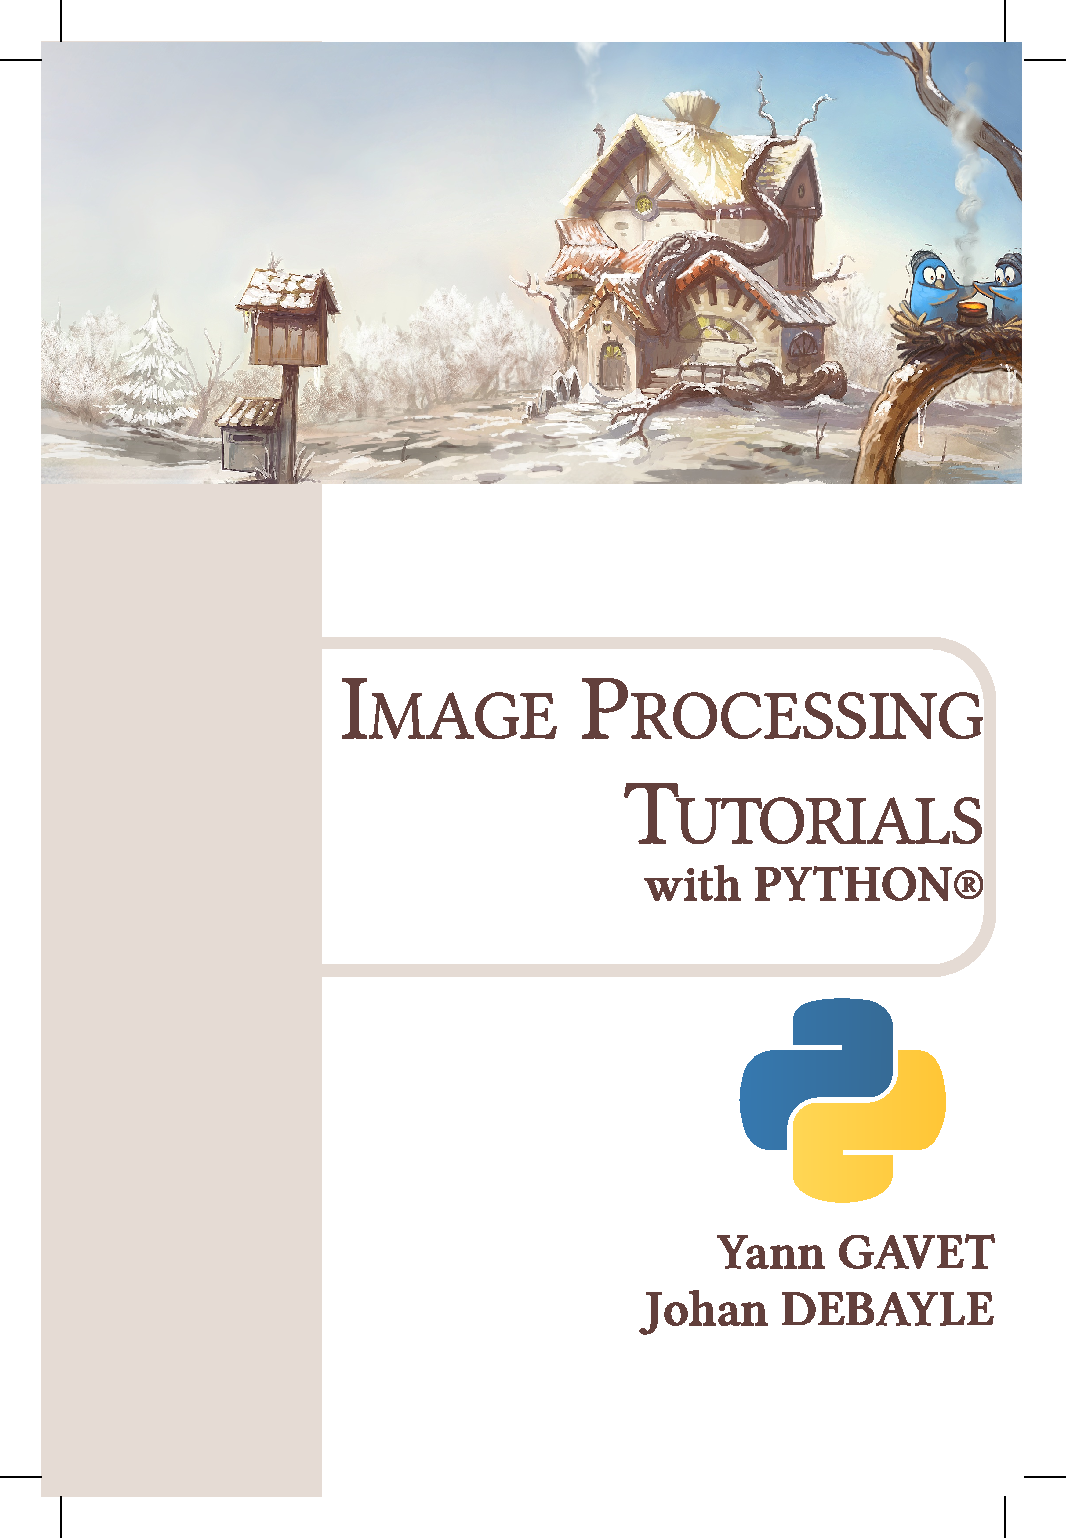
\includepdf[pages={1},fitpaper]{media/TUT_pagedegarde_python_16x24.pdf}
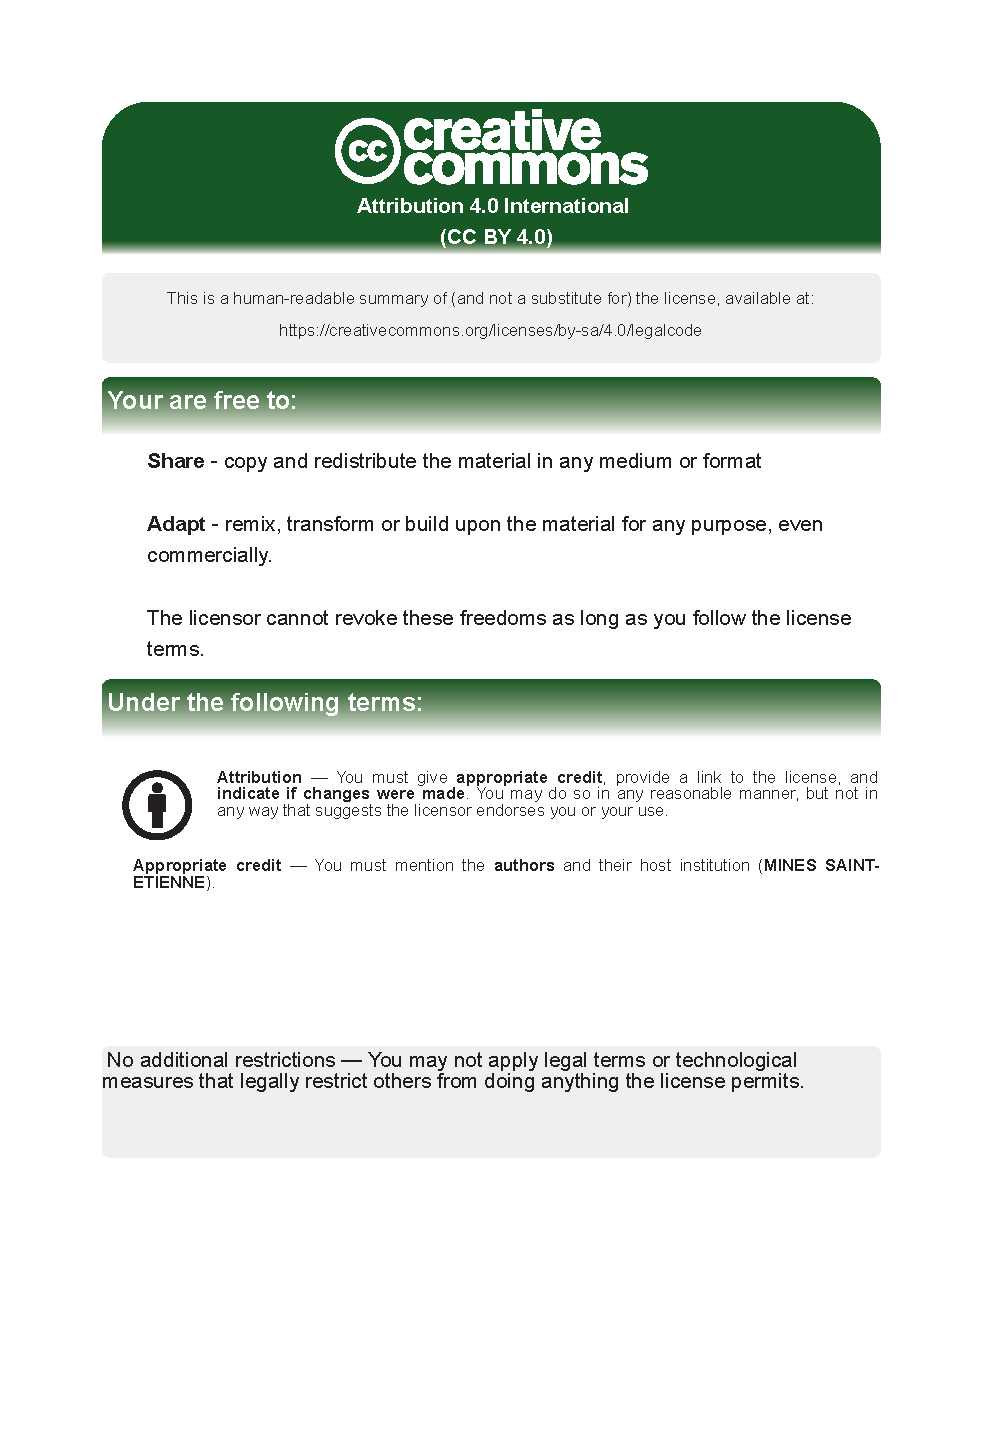
\includepdf[pages={1},fitpaper]{media/license_16x24.pdf}
\tableofcontents
\section*{About the authors}
\subsection*{Yann GAVET}

received his "Ingénieur Civil des Mines de Saint-Etienne" diploma in 2001. He then obtained a Master of Science and a PhD thesis on the segmentation of human corneal endothelial cells (in 2004 and 2008). He is now an assistant professor at the Saint-Etienne School of Mines, where he teaches computer science and image processing to engineering and master students. He is a member of the PMDM Department of the LGF Laboratory, UMR CNRS 5307, dedicated to granular media analysis and modelisation.

He is particularly interested in the world of free (LIBRE) software in computer science. His research interests include image processing and analysis, stochastic geometry and numerical simulations. He published more than 70 papers in international journals and conference proceedings. He is a member of the Institute of Electrical and Electronics Engineers (IEEE), the International Association for Pattern Recognition (IAPR), International Society for Stereology and Image Analysis (ISSIA). He has worked for CS-SI (Toulouse, France) as an IT engineer, and for Thalès-Angénieux (Saint-Héand, France) as an image processing expert.

\subsection*{Johan DEBAYLE} 

received his M.Sc., Ph.D. and Habilitation degrees in the field of image processing and analysis, in 2002, 2005 and 2012 respectively. Currently, he is a Full Professor at the Ecole Nationale Supérieure des Mines de Saint-Etienne (ENSM-SE) in France, within the SPIN Center and the LGF Laboratory, UMR CNRS 5307, where he leads the PMDM Department interested in image analysis of granular media. In 2015, he was a Visiting Researcher for 3 months at the ITWM Fraunhofer / University of Kaisersleutern in Germany. In 2017 and 2019, he was invited as Guest Lecturer at the University Gadjah Mada, Yogyakarta, Indonesia. He was also Invited Professor at the University of Puebla in Mexico in 2018 and 2019. He is the Head of the Master of Science in Mathematical Imaging and Spatial Pattern Analysis (MISPA) at the ENSM-SE.

His research interests include image processing and analysis, pattern recognition and stochastic geometry. He published more than 120 international papers in international journals and conference proceedings and served as Program committee member in several international conferences (IEEE ICIP, MICCAI, ICIAR…). He has been invited to give a keynote talk in several international conferences (SPIE ICMV, IEEE ISIVC, SPIE-IS\&T EI, SPIE DCS…)
He is Associate Editor for 3 international journals: Pattern Analysis and Applications (Springer), Journal of Electronic Imaging (SPIE) and Image Analysis and Stereology (ISSIA).

He is a member of the International Society for Optics and Photonics (SPIE), International Association for Pattern Recognition (IAPR), International Society for Stereology and Image Analysis (ISSIA) and Senior Member of the Institute of Electrical and Electronics Engineers (IEEE). 

\subsection*{\'ECOLE NATIONALE SUP\'ERIEURE DES MI\-NES DE SAINT-\'ETI\-EN\-NE}

One of the missions of École des Mines de Saint-Étienne, France, is scientific research at the highest level and contributions to companies’ competitiveness. It aims at conveying the economical politics of the country and speeding up the sustainable industrial development by innovation and efficient contributions.

This high level scientific research leads to publications recognized  by the international scientific community. Research and teaching are very closely interwoven and the consequence of this is the attractiveness of our Master’s Degree courses and our renowned Doctoral School.

\begin{center}
 
\includegraphics[width=7cm]{emse.pdf}
\end{center}
% 
% \subsection*{Why a CC-By license?}
% The CC-by license is a very unrestrictive license. In particular, it authorizes everyone to reuse the document, to distribute it, even commercially, on the sole condition that the authors are cited. So why would we do that?  
% 
% What we believe is important is to distribute knowledge freely. Our names on the book are more than enough. If the reader can say after studying these pages: "we really do interesting things in Saint-Etienne", well, the objective will be achieved. Our salaries are paid by the French government, we are teacher-researchers, this work belongs to the public. Our hope is that it will serve some people.

\newpage
\begin{figure}
 \centering
\EANisbn
\end{figure} 
 
\newpage
\part{Premi\`ere partie: \matlabregistered}
\def\difficulty{3} 
\chapter[Chapitre super long]{Ceci est un nom de Chapitre super long super super super super} 

\begin{note}Ceci est une note!\end{note}

\begin{rmq} 
 Ceci est une remarque.
\end{rmq}

\mcorrectionsection{Matlab correction} 

\sujet{Ceci est un sujet}

\def\difficulty{1}
\sujet{Introduction to image processing}


\begin{note}
In this tutorial, you will discover the basic functions in order to load, manipulate and  display images. The main informations of the images will be retrieved, like size, number of channels, storage class, etc. Afterwards, you will be able to perform your first classic filters.
\end{note}

\noindent The different processes will be realized on the following images:

\vspace*{-8pt}
\begin{figure}[htbp]
\centering\caption{Image examples.}
\subfloat[Retinal vessels.]{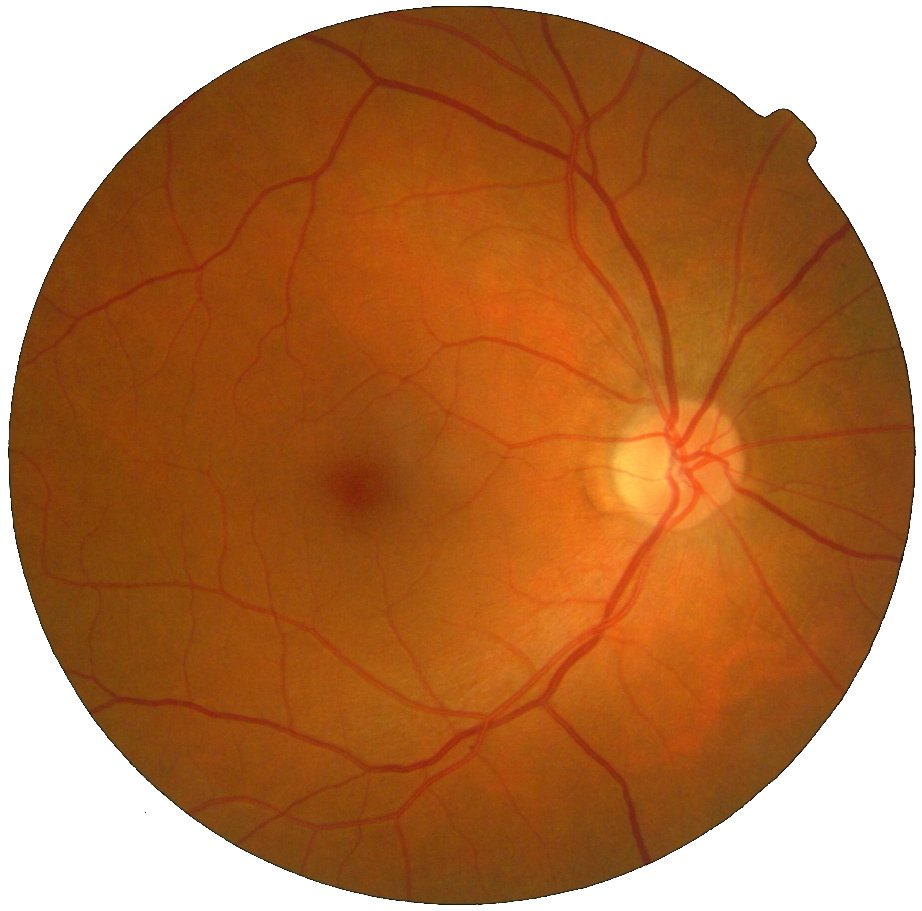
\includegraphics[height=.28\linewidth]{retine.png}}
\hfill
\subfloat[Muscle cells.]{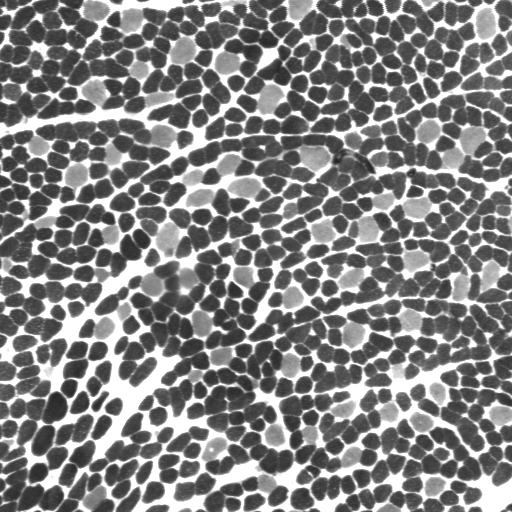
\includegraphics[height=.3\linewidth]{muscle.jpg}}
\hfill
\subfloat[Cornea cells (BIIGC, Univ. Jean Monnet, Saint-Etienne, France).]{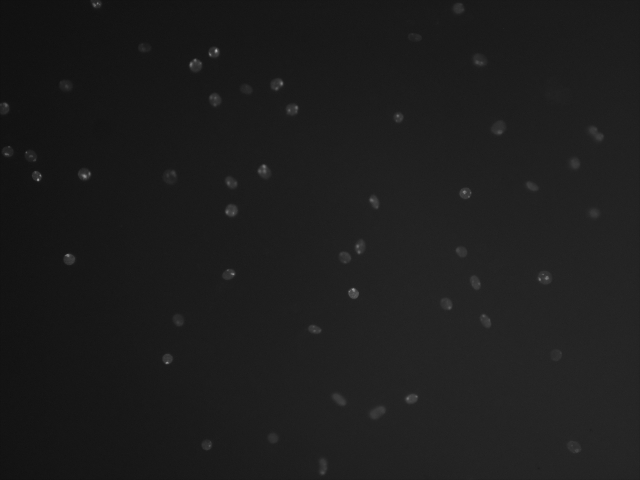
\includegraphics[height=.3\linewidth]{cellules_cornee.jpg}}
\vspace*{-10pt}
\end{figure}

\vspace*{-15pt}

%%%%%%%%%%%%%%%%%%%%%%%%%%%%%%%%%%%%%%%%%%%%%%%%%%%%%%%%%%%%%%%%%%%%%%%%%%%%%%%%%%%%%%%%

\section{First manipulations}
\index{Image!Load}\index{Image!Display}

\begin{pcomment}
\begin{premark}Image loading can be made by the use of the python function \pinline{imageio.imread}.
The visualization of the image in the screen is realized by using the module \pinline{matplotlib.pyplot}.
\end{premark}
\end{pcomment}

\begin{mcomment}
\begin{mremark}Image loading can be made by the use of the \matlabregistered{} function \minline{imread}. 
The visualization of the image in the screen is realized either by the \matlabregistered{} function \minline{imagesc} or \minline{imshow}.
\end{mremark}
\end{mcomment}

\begin{qbox}
\begin{itemize}
\item Load and visualize the first image as below. Notice the differences.
 \item Look at the data structure of the image $I$ such as its size, type\dots.
\item Visualize the green component of the image.
Is it different from the red one? What is the most contrasted color component? Why? 
\item Enumerate some digital image file formats. 
What are their main differences? 
Try to write images with the JPEG file format with different compression ratios (0, 50 and 100), as while as the lossless compression, and compare.
\end{itemize}
\end{qbox}

\begin{mcomment}
 \begin{mremark}
  See \minline{imwrite}.
 \end{mremark}
\end{mcomment}

%%%%%%%%%%%%%%%%%%%%%%%%%%%%%%%%%%%%%%%%%%%%%%%%%%%%%%%%%%%%%%%%%%%%%%%%%%%%%%%%%%%%%%%%%%%%%%%%%%%
\section{Color quantization}
\index{Quantization}
Color quantization is a process that reduces the number of distinct colors used in an image, usually with the intention that the resulting image should be as visually similar as possible to the original image. In principle, a color image is usually quantized with 8 bits (i.e. 256 gray levels) for each color component.

\begin{qbox}
\begin{itemize}
\item By using the gray level image 'muscle', reduce the number of gray levels to  128, 64, 32, and visualize the different resulting images.
\item Compute the different image histograms and compare. 
\end{itemize}
\end{qbox}



%%%%%%%%%%%%%%%%%%%%%%%%%%%%%%%%%%%%%%%%%%%%%%%%%%%%%%%%%%%%%%%%%%%%%%%%%%%%%%%%%%%%%%%%%%%%%%%%%%%
\vspace*{-8pt}
\section{Image histogram}
\index{Histogram}
An image histogram represents the gray level distribution in a digital image.
The histogram corresponds to the number of pixels for each gray level.
\begin{mcomment}
The \matlabregistered{} function that computes the histogram of any gray level image has the following prototype:
\begin{matlab}
function h = histogram(I)
\end{matlab}
\end{mcomment}

\begin{pcomment}
The python function has the following prototype:
\begin{python}
def histogram(I):
\end{python}
\end{pcomment}

\begin{qbox}
Compute and visualize the histogram of the image 'muscle.jpg'.
\end{qbox}


%%%%%%%%%%%%%%%%%%%%%%%%%%%%%%%%%%%%%%%%%%%%%%%%%%%%%%%%%%%%%%%%%%%%%%%%%%%%%%%%

\vspace*{-8pt}
\section{Linear mapping of the image in\-ten\-si\-ties}

The gray level range of the image 'cellules\_cornee.jpg' can be enhanced by a linear map\-ping such that the minimum (resp. maximum) gray level value of the resulting image is $0$ (resp. $255$). Mathematical\-ly, it consists in finding a function $f(x)=ax+b$ such that 
$f(min)=0$ and $f(max)=255$.

\begin{qbox}
\begin{itemize}
\item Load the image and find its extremal gray level values.
\item Adjust the intensities by a linear mapping into $[0, 255]$.

\item Visualize the resulting image and its histogram.
\end{itemize}
\end{qbox}

\vspace*{-8pt}

\section{Aliasing effect}
\index{Aliasing}

\begin{qbox}
	\begin{minipage}{0.6\textwidth}
\begin{itemize}
\item Create an image (as right) that contains rings as sinusoids. The function takes two input parameters: the sampling frequency and the signal frequency.
%\begin{center}
%
\includegraphics[height=3.5cm]{moire.png}
%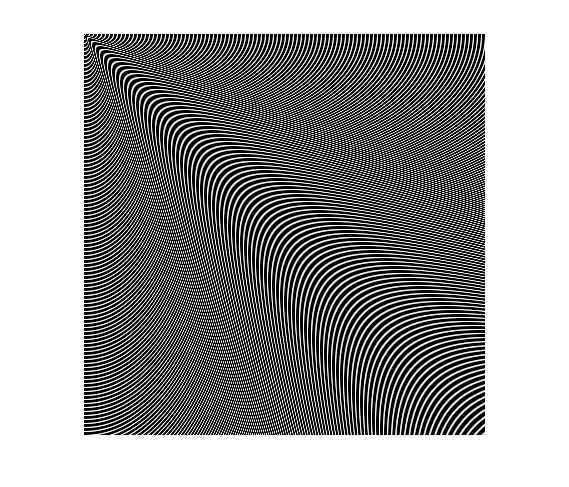
\includegraphics[height=4.25cm]{moire2.png}
%\end{center}
\item Look at the influence of the two varying frequencies. What do you observe? Explain the phenomenon from a theoretical point of view.
\end{itemize}
\end{minipage}
\hfill
\begin{minipage}{0.35\textwidth}
	
\includegraphics[height=3.5cm]{moire.png}
\end{minipage}
\end{qbox}

%%%%%%%%%%%%%%%%%
% filtering


\section{Low-pass filtering}
\index{Filtering!Low-pass}\index{Filtering!Convolution}

The different processes will be realized on the following images:
{
	\makeatletter
	\renewcommand\fs@ruled{\def\@fs@cfont{\bfseries}\let\@fs@capt\floatc@ruled
		\def\@fs@pre{\hrule height.8pt depth0pt \kern2pt}%
		\def\@fs@post{\kern2pt\hrule\relax}%
		\def\@fs@mid{\vskip2pt}%
		\let\@fs@iftopcapt\iftrue}
	\makeatother
\begin{figure}[H]
\centering
\subfloat[osteoblast cells]{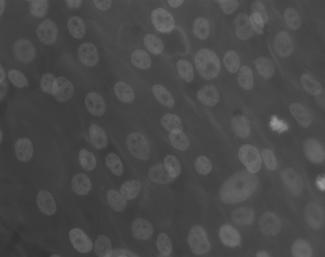
\includegraphics[height=4.5cm]{osteoblaste.jpg}}
\hfill
\subfloat[blood cells]{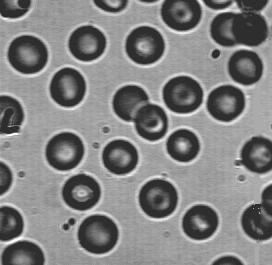
\includegraphics[height=4.5cm]{blood.jpg}}
\vspace*{-10pt}
\end{figure}
}

Low-pass filtering aims to smooth the fast intensity variations of the image to be processed.
\begin{qbox}
Test the low-pass filters 'mean', 'median', 'min', 'max' and 'gaussian' on the noisy image 'blood cells'. 
\end{qbox}

	\begin{mcomment}
\begin{mremark}The \matlabregistered{} functions \minline{imfilter} and \minline{nlfilter} can be employed.
Be careful to the function options for border problems. Also, the \matlabregistered{} function \minline{fspecial} enables an operational window to be generated.
\end{mremark}
\end{mcomment}

\begin{pcomment}
\begin{premark}
The module \pinline{scipy.ndimage.filters} contains a lot of classical filters.
\end{premark}
\end{pcomment}
\begin{qbox}
Which filter is suitable for the restoration of this image?
\end{qbox}

%%%%%%%%%%%%%%%%%%%%%%%%%%%%%%%%%%%%%%%%%%%%%%%%%%%%%%%%%%%%%%%%%%%%%%%%%%%%%%%%%%%%%%%%%%%%%%%%%%%
\section{High-pass filtering}
\index{Filtering!High-pass}
\index{Laplacian}

High-pass filtering aims to smooth the low intensity variations of the image to be processed.
\begin{qbox}
\begin{itemize}
	\item Test the high-pass filters $HP$ on the two initial images in the following way: 
	$HP(f)=f-LP(f)$ where $LP$ is a low-pass filtering (see the previous exercise).
	\item Test the Laplacian \label{lbl:introduction:laplacien}(high-pass) filter on the two initial images with the following convolution mask:
$$
\left[
\begin{array}{ccc}
-1&-1&-1\\
-1&+8&-1\\
-1&-1&-1
\end{array}
\right]
$$
\end{itemize}
\end{qbox}


\section{Derivative filters}
\index{Gradient!Prewitt}
\index{Gradient!Sobel}

Derivative filtering aims to detect the edges (contours) of the image to be processed.
\begin{qbox}
\begin{itemize}
	\item
Test the Prewitt and Sobel derivative filters (corresponding to first order derivatives) on the image 'blood cells' with the use of the following convolution masks:
$$
\left[
\begin{array}{ccc}
-1&0&+1\\
-1&0&+1\\
-1&0&+1
\end{array}
\right]
\left[
\begin{array}{rrr}
-1&-1&-1\\
0&0&0\\
+1&+1&+1
\end{array}
\right]
$$
$$
\left[
\begin{array}{ccc}
-1&0&+1\\
-2&0&+2\\
-1&0&+1
\end{array}
\right]
\left[
\begin{array}{rrr}
-1&-2&-1\\
0&0&0\\
+1&+2&+1
\end{array}
\right]
$$
\item Look at the results for the different gradient directions.
\item Define an operator taking into account the horizontal and vertical directions.
\end{itemize}
\end{qbox}

Remark : the edges could be also detected with the zero-cressings of the Laplacian filtering  (corresponding to second order derivatives).

 

\section{Enhancement filtering}
Enhancement filtering aims to enhance the contrast or accentuate some specific image characteristics.
\begin{qbox}
\begin{itemize}
	\item Test the enhancement filter $E$ on the image 'osteoblast cells' defined as:
	$E(f)=f+HP(f)$ where $HP$ is a Laplacian filter (see  \iflabelexists{tutorial:image_enhancement}{tutorial \ref{tutorial:image_enhancement}.}{tutorial about enhancement.}).
	\item Parameterize the previous filter as:
	$E(f)=\alpha f+HP(f)$, where $\alpha\in\mathbb{R}$.
\end{itemize}
\end{qbox}

\section{Open question}
Find an image filter for enhancing the gray level range of the image 'osteoblast cells'.


\newpage
\inputmatlabcorrection{../TB_image/TUT.IMG.introduction/matlab/text.tex}
\inputpythoncorrection{../TB_image/TUT.IMG.introduction/python/text.tex}

\sujet[Option du sujet]{Ceci est un sujet}
\section{section}
\section{Ceci est un titre de section supersuper long qui dépasse la ligne}
\subsection{subsection}
\subsubsection{subsubsection}

\begin{matlab}
function t = test(A)
% this is a test function
A = rand(25,2);
imagesc(A);
[X, Y] = meshgrid(1:10, 1:10);
\end{matlab}

\begin{python}
def myFunction(toto):
	# this is a test function
	return True;
\end{python}

\mcorrectionsection{Matlab correction}
\begin{mwindow}
 test
\end{mwindow}

\subsection{subsection}
\subsection{Matlab environments}
Deux environnements doivent être présentés maintenant, sauf si excludecomment est utilisé:

\begin{mcomment}

\begin{mremark}
This is a \matlabregistered{} mremark environment.
\end{mremark}

\end{mcomment}

\begin{mhelp}
This is a \matlabregistered{} mhelp. 

\lipsum[1-2]
\end{mhelp}


Voilà, c'est fait.

\pcorrectionsection{Python correction}
\begin{sh}
This is a shell to show python results.
\end{sh}
 
\subsection{subsection}
\subsection{Python environments}

\begin{pcomment}

\begin{premark}
This is a python premark environment.
\end{premark}

\end{pcomment}


\begin{phelp}
 This is a python phelp environment
\end{phelp}

\begin{qbox}
 this is a serie of questions, available with qbox.
\begin{itemize}
\item ATTENTION: L'UTILISATION DE PLUSIEURS PAGES SEMBLENT POSER PRO\-BLÈME.
 \item \lipsum[1]
 \item \lipsum[1-2]
\end{itemize}
\end{qbox}


\lipsum[1]

\section{Test existence of label}
\iflabelexists{fig:test}{Label ``fig:test'' exists!}{Label ``fig:test'' does'nt exist! New label: \ref{fig:test2}.
\begin{figure}
 \centering
 
\includegraphics[width=1cm]{media/python-logo.pdf}
 \caption{Figure example}
 \label{fig:test2}
\end{figure}
} % iflabelexists

\def\difficulty{2}
\chapter[2e chapitre long]{Ceci est encore un nom de Chapitre su\-per\-su\-per long}


\section{section}
\section{section}
\section{section}
\section{section}
\section{section}
\section{section}
\section{section}
\section{section}
\section{section}
\section{section}
\section{section}
\section{section}
\section{section}
\section{section}
\section{section}
\section{section}
\section{section}
\section{section}

\addtocontents{toc}{\protect\newpage}
\part{2nd part}
\chapter{Chapitre}
\chapter{New chapter}
 \section{sec of new chapter}
 
\chapter{New chapter}
\chapter{New chapter}
\chapter{New chapter}
\chapter{New chapter}
\chapter{New chapter}
\chapter{New chapter}
\chapter{New chapter}
\chapter{New chapter}
\chapter{New chapter}
\chapter{New chapter}
 \section{sec of new chapter}\lipsum[1-5]
 \section{sec of new chapter}
\lipsum[1-5]

\apppart{References}


\newpage
% 4e de couverture
\textbf{Image processing tutorials with python}
This book is a collection of tutorials and exercises given at MINES Saint-Etienne as part of the Master’s Degree in Science and Executive Engineering ("Ingénieur Civil des Mines -- ICM"). In recent years, project-based learning has been used to illustrate theoretical concepts with real and concrete applications.

Whether you are in the early years of your university studies, in preparatory classes for the French Grandes Ecoles or in an engineering school, or even as a teacher, this book is made for you. You will find a large number of tutorials, classified by field, to familiarize yourself with the theoretical concepts of image processing and analysis. 

Go to http://iptutorials.science to download the complete codes in python.

\textbf{Yann GAVET} He graduated from Mines Saint-Etienne with a Master’s Degree in Science and Executive Engineering ("Ingénieur Civil des Mines - ICM") in 2001, obtained a Master of Science in 2004 and defended his PhD thesis in 2008. He teaches signal-processing, image-processing and pattern-recognition as well as C programming at Master’s level.

\textbf{Johan DEBAYLE} He received his master of science and PhD thesis in 2002 and 2005. He is the head of the master MISPA of MINES Saint-\'Etienne, and teaches signal-processing, image-processing and pattern-recognition at Master's level.

\begin{center}
 
\includegraphics[width=3cm]{emse.pdf}
\end{center}

\end{document}
